\documentclass{article}
\usepackage{amsmath}
\usepackage{graphicx}
\title{Mock Interview: Machine Learning}
\date{}
\begin{document}
\maketitle

What is Linear Regression?
\newpage
I have a data matrix \textbf{X} $\in n\text{ x }d $ where $n$ is the size of the training data
		and $d$ is the dimension of the data.  Let's call the model parameter \textbf{w}, and the target \textbf{y}.
		What are the dimensions of \textbf{w} and \textbf{y}?
\newpage
Assume that $\textbf{d} = 1$.  Solve of \textbf{w} in terms of \textbf{y} and \textbf{x}.
\\ \\ \\ \\ \\ \\ \\ \\ \\ \\ \\
\\ \\ \\ \\ \\ \\ \\ \\ \\ \\ \\
\vspace{3cm} 
HINTS: 
\begin{itemize}
		\item What's the dimension of \textbf{X}?  What is the dimension of \textbf{w}?
		\item Let's call them \textbf{x} (since it is an $n \text{ x } 1$ vector) and $w$ (since it is a scalar).
		\item What's the loss function you want to optimize for?  (Squared loss).  Write out the loss function.
		\item What are you optimizing it with respect to?

		\item $\text{minimize}_\textbf{w} ||\textbf{x}w - \textbf{y}||_2^2$ is the optimization problem.  Now take the derivative, set it to zero and solve for $w$.  You will arrive at $w = \frac{\textbf{x}^T\textbf{y}}{\textbf{x}^T\textbf{x}}$.
\end{itemize}
				\newpage
Can you generalize your solution $w = \frac{\textbf{x}^T\textbf{y}}{\textbf{x}^T\textbf{x}}$ to case where $\textbf{d} > 1$?  
\\ \\ \\ \\ \\ \\ \\ \\ \\ \\ \\
\\ \\ \\ \\ \\ \\ \\ \\ \\ \\ \\
\[
		\textbf{w} = {(\textbf{X}^T\textbf{X})}^{-1} \textbf{X}^T\textbf{y}.
\]
Briefly ask about the matrix inversion.
\vspace{3cm} 
\newpage
Let's go back to your loss function.  Is your loss function missing anything?
\\ \\ \\ \\ \\ \\ \\ \\ \\ \\ \\
\\ \\ \\ \\ \\ \\ \\ \\ \\ \\ \\

HINTS:  Regularization.  Trade of between model complexity and minimizing the loss.
\newpage
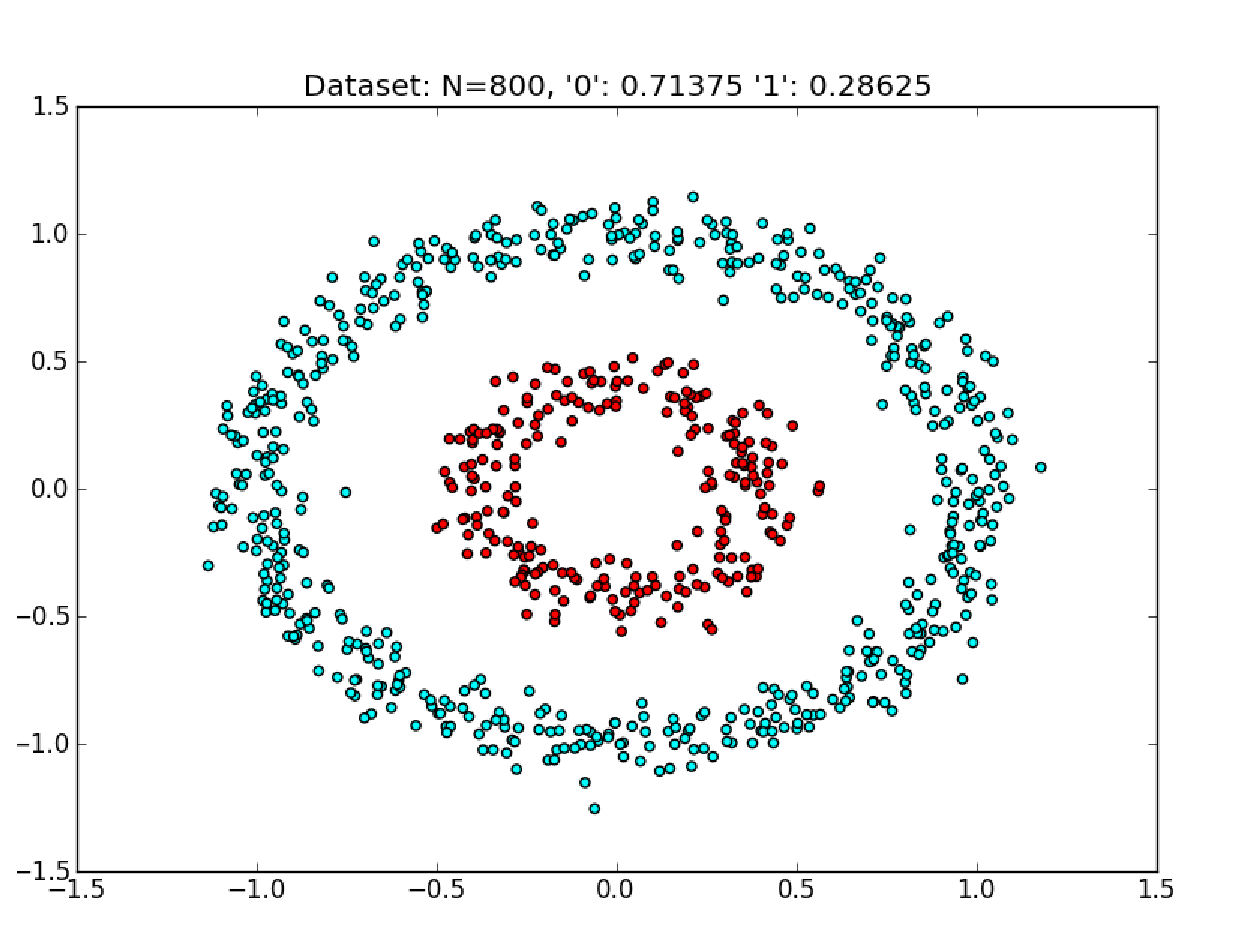
\includegraphics[width=\textwidth]{dataset_nonsep}
Consider the plot above.  Will linear regression be a good model for the data below?  Explain your answer.
\end{document}
